\documentclass[11pt]{report}
\usepackage{textcomp}

\usepackage{titlesec}
\titlespacing*{\section}
{0pt}{\baselineskip}{0em}
\titlespacing*{\subsection}
{0pt}{\baselineskip}{0em}

\usepackage{geometry}
\geometry{left=1in, right=1in, top=1in, textheight=9in}

\usepackage{enumitem}
\newlist{steps}{enumerate}{1}
\setlist[steps, 1]{wide=0pt, leftmargin=\parindent, label=Step \arabic*:}

\usepackage{fancyhdr}
\fancypagestyle{plain}{%
    \fancyhf{} % clear all header and footer fields
    \fancyfoot[C]{\sffamily\fontsize{.75em}{.75em}\selectfont\thepage} % except the center
    \renewcommand{\headrulewidth}{0pt}
    \renewcommand{\footrulewidth}{0pt}
}
\pagestyle{plain}

\usepackage{graphicx}
\graphicspath{ {./media/} }

\usepackage{setspace}
\doublespacing

\usepackage{minted}
\usepackage{xcolor}
\definecolor{LightGray}{gray}{0.9}

% make fancy title page
\makeatletter
\newcommand{\@labsection}{000}
\newcommand{\labsection}[1]{
    \renewcommand{\@labsection}{#1}
}

\newcommand{\@labnumber}{0}
\newcommand{\labnumber}[1]{
    \renewcommand{\@labnumber}{#1}
}

\newcommand{\@shortsubmitted}{1/1/70}
\newcommand{\shortsubmitted}[1]{
    \renewcommand{\@shortsubmitted}{#1}
}

\lfoot{\footnotesize \textit{University of Arkansas \\ EECS Department}}
\rfoot{\footnotesize \textsl{\@shortsubmitted}}

\renewcommand{\maketitle}{
    \newgeometry{left=1in, right=1in, top=1.75in, textheight=8.25in}
    \singlespacing
    \begin{center}
        {\huge \bf CSCE 22104} \\
        \vspace{2.5em}
        {\Large \bf Lab Report} \\
        \vspace{2em}
        \noindent\rule{20em}{0.4pt} \\
        \vspace{1em}
        {\Large \@author} \\
        \vspace{.75em}
        {\normalsize ID: 011019116} \\
        \vspace{.75em}
        {\normalsize Lab Section \@labsection} \\
        \vspace{.75em}
        {\normalsize Lab \@labnumber} \\
    \end{center}
    \newpage
    \restoregeometry
}

\makeatother


% TEXTWIDTH = 100
\begin{document}
\title{Lab Report 7}
\author{Brent Marcus Orlina}

\labsection{001}
\labnumber{7}

\shortsubmitted{4/2/25}

\maketitle

\section*{Introduction}
This lab's goal was to implement a register file and CPU component from a given template. The
register file should be able to hold 16-bit data with a total of 16 registers, making the register
addresses 4-bits in length. The CPU component should take in a 16-bit instruction, with the first
four bits representing the opcode, the second four bits representing the register destination
\verb|rd|, and the third and fourth four bits representing the operand registers \verb|rs| and
\verb|rt|. The ALU used in the CPU is from Lab 6, still supporting only four operations, meaning
that the first two bits of the opcode is unused.

\newpage

\section*{Approach}
\begin{listing}[h!]
    \inputminted[
        frame=lines,
        breaklines,
        linenos,
        tabsize=4,
        fontsize=\footnotesize,
        bgcolor=LightGray
    ]{vhdl}{./media/regfile-port.vhd}
    \caption{The register file component's ports.}
    \label{listing:regfile-port}
\end{listing}

The register file was first implemented. Listing \ref{listing:regfile-port} shows the ports that the
register file has. Since the CPU is synchronized, the register file needs to a clock, represented by
the input port \verb|clk|. The input port \verb|clear| resets all the registers in the register file
to $0$, with the exception of register 1, which always holds $1$. The input ports \verb|write_addr|,
\verb|write_data|, \verb|load| is for writing data into the register file. The input port
\verb|load| determines whether the data in \verb|write_data| should be loaded into
\verb|write_addr|. Input ports \verb|read_addr1| and \verb|read_addr2| are the register addresses to
be read, with the data being outputted to the output ports \verb|read_data1| and \verb|read_data2|
respectively.

\begin{listing}[ht!]
    \inputminted[
        frame=lines,
        breaklines,
        linenos,
        tabsize=4,
        fontsize=\footnotesize,
        bgcolor=LightGray
    ]{vhdl}{./media/regfile-architecture.vhd}
    \caption{The register file component's architecture.}
    \label{listing:regfile-architecture}
\end{listing}

Listing \ref{listing:regfile-architecture} shows the implementation of the register file. The data
is stored in a signal of an array of 16-bit vectors with a total of 16 registers. The process of
writing to and clearing the register file is sensitive to the ports \verb|clk|, \verb|load|, and
\verb|clear|. The input port \verb|clear| is low active asynchronous, meaning that the registers are
resetted to zero independent of the clock if \verb|clear| is inactive. The data in the port
\verb|write_data| is written to the register determined by the port \verb|write_addr| if the clock
is in a rising edge and if \verb|load| is active as seen on line 12. On lines 15 and 16, it is
ensured that registers 0 and 1 always hold the values 0 and 1 respectively, so that even if it is
attempted to write to those registers, those registers will not be mutated. Finally, on lines
registers 18 and 19, the output ports \verb|read_data1| and \verb|read_data2| are set to the values
stored in the register addresses in \verb|read_addr1| and \verb|read_addr2| respectively. These are
not in the process since they do not need to be synchronous to the clock nor do they depend on the
\verb|load| signal or \verb|clear| signal.

\newpage

\begin{listing}[ht!]
    \inputminted[
        frame=lines,
        breaklines,
        linenos,
        tabsize=4,
        fontsize=\footnotesize,
        bgcolor=LightGray
    ]{vhdl}{./media/CPU-port.vhd}
    \caption{The CPU component's ports.}
    \label{listing:CPU-port}
\end{listing}

Listing \ref{listing:CPU-port} shows the ports for the CPU component. The input port \verb|clk| is
to synchronize the instructions that the CPU is fed. The input port \verb|clear| is to reset the
register file. Finally the input port \verb|instruction| determines what the CPU does. The first
four bits representing the opcode, the second four bits representing the register destination
\verb|rd|, and the third and fourth four bits representing the operand registers \verb|rs| and
\verb|rt|.

%
% \newpage
% \begin{listing}[ht!]
%     \inputminted[
%         frame=lines,
%         breaklines,
%         linenos,
%         tabsize=4,
%         fontsize=\footnotesize,
%         bgcolor=LightGray
%     ]{vhdl}{./media/CPU-components.vhd}
%     \caption{The components that the CPU implementation uses.}
%     \label{listing:CPU-components}
% \end{listing}
% 
% Listing \ref{listing:CPU-components} shows the components that the CPU implementation uses. It uses
% a 16-bit ALU and the recently implemented register file. 

\newpage

\begin{listing}[ht!]
    \inputminted[
        frame=lines,
        breaklines,
        linenos,
        tabsize=4,
        fontsize=\footnotesize,
        bgcolor=LightGray
    ]{vhdl}{./media/CPU-signals.vhd}
    \caption{The signals that the CPU implementation uses.}
    \label{listing:CPU-signals}
\end{listing}

Listing \ref{listing:CPU-signals} shows the signals used in the implementation. The signals
\verb|OP|, \verb|RS|, \verb|RT|, and \verb|RD| is used to separate the instruction to their
representative sections. The signals \verb|RSData| and \verb|RTData| are used to connect the outputs
of the reads from the register to the ALU. The signals \verb|cout| and \verb|Sout_ALU| are used for
the outputs of the ALU, where \verb|cout| is the final carry out and \verb|Sout_ALU| is the result
of the ALU, eventually writing back to the register file.

\begin{listing}[h!]
    \inputminted[
        frame=lines,
        breaklines,
        linenos,
        tabsize=4,
        fontsize=\footnotesize,
        bgcolor=LightGray
    ]{vhdl}{./media/CPU-fetch.vhd}
    \caption{The instruction fetch phase of the CPU implementation.}
    \label{listing:CPU-fetch}
\end{listing}

Listing \ref{listing:CPU-fetch} shows the instruction fetch phase of the CPU implementation. This
phase simply splits the instruction into its respective parts.

\newpage

\begin{listing}[h!]
    \inputminted[
        frame=lines,
        breaklines,
        linenos,
        tabsize=4,
        fontsize=\footnotesize,
        bgcolor=LightGray
    ]{vhdl}{./media/CPU-decode.vhd}
    \caption{The instruction decode phase of the CPU implementation.}
    \label{listing:CPU-decode}
\end{listing}

Listing \ref{listing:CPU-decode} shows the instruction decode phase of the CPU implementation. This
connects the respective \verb|clk| and \verb|clear| signals to the register file as well as the
register signals to the register file. The register signals, \verb|RS| and \verb|RT| is as the read
addresses of register file, with the register contents going to the signals \verb|RSData| and
\verb|RTData|. The \verb|RD| signal is used as the write address with the output of the ALU, the
\verb|Sout_ALU| signal, being written to that address. The input port \verb|load| of the register
file is always active since all of the instructions supported by the CPU implementation currently
always writes back to the register file. Since this section also shows writing to the register, it
can also be considered to be the write-back phase of the CPU implementation.

\newpage

\begin{listing}[h!]
    \inputminted[
        frame=lines,
        breaklines,
        linenos,
        tabsize=4,
        fontsize=\footnotesize,
        bgcolor=LightGray
    ]{vhdl}{./media/CPU-execute.vhd}
    \caption{The instruction execution phase of the CPU implementation.}
    \label{listing:CPU-execute}
\end{listing}

Listing \ref{listing:CPU-execute} shows the execution phase. It connects the data read from the
register file, in the signals \verb|RSData| and \verb|RTData|, to the 16-bit ALU implemented from a
previous lab. It also notable connects the only the two lower bits of the opcode. This is because
the CPU still only supports four instructions, thus the ALU only needs two bits with the two higher
bits of the opcode being unused. The two higher bits will be used to implement future instructions.
Finally, the result of the ALU is connected to \verb|Sout_ALU|, which is connected back to the
register file for writing, and the carry out of the ALU is connected to \verb|cout| so that it can
be observed.

\section*{Experimentation}
The components were tested by writing a testbench for the CPU component. The testbench written
tested for given instructions for the CPU and were manually verified to be correct.

\newpage

\section*{Results \& Discussion}
\begin{figure}[h!]
    \centering
    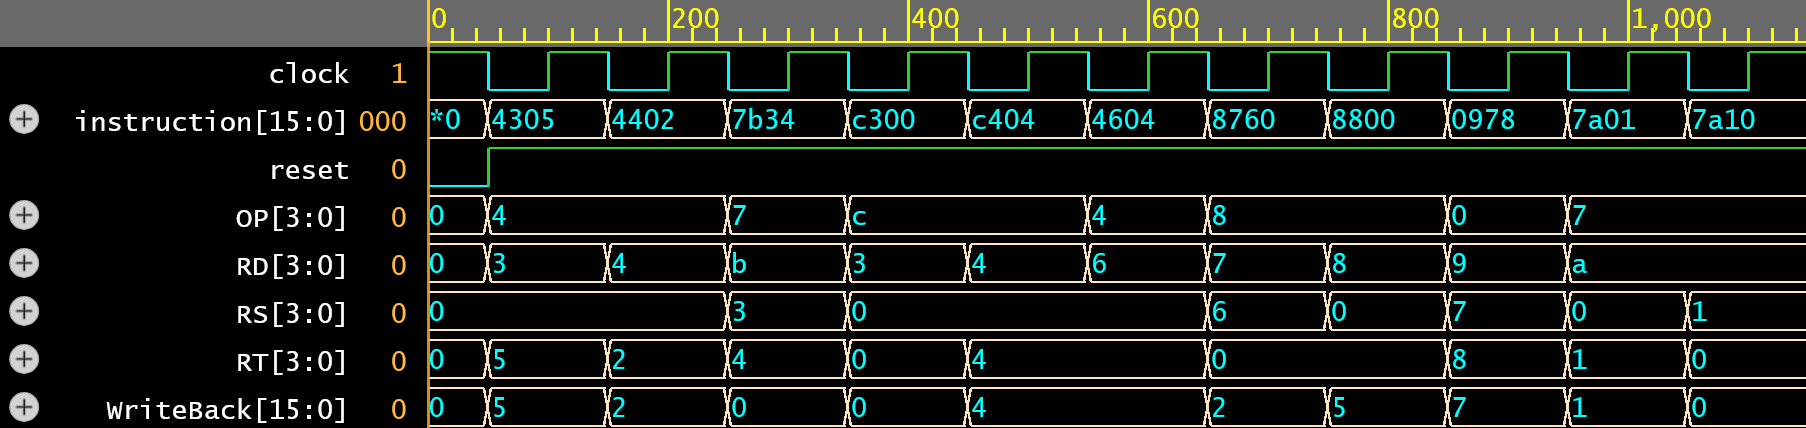
\includegraphics[width=0.95\textwidth]{CPU-waveform}
    \caption{The waveform for the CPU component.}
    \label{fig:CPU-waveform}
\end{figure}

\begin{table}[ht!]
    \centering
    \begin{tabular}{|l||c|c|c|c|c|} 
     \hline
     Instruction & op & rd & rs & rt & value (of rd) \\
     \hline
     \verb|ADD R2, R1, R1| & \verb|0x0| & \verb|0x2| & \verb|0x2| & \verb|0x1| & \verb|2| \\ 
     \hline                                                                             
     \verb|ADD R3, R2, R1| & \verb|0x0| & \verb|0x3| & \verb|0x2| & \verb|0x1| & \verb|3| \\
     \hline                                                                             
     \verb|ADD R4, R3, R2| & \verb|0x0| & \verb|0x4| & \verb|0x3| & \verb|0x2| & \verb|5| \\
     \hline                                                                             
     %
     \verb|SUB R5, R4, R3| & \verb|0x1| & \verb|0x5| & \verb|0x4| & \verb|0x3| & \verb|2| \\ 
     \hline                                                                             
     \verb|SUB R1, R5, R1| & \verb|0x1| & \verb|0x1| & \verb|0x5| & \verb|0x1| & \verb|1| \\
     \hline                                                                             
     \verb|SUB R0, R3, R0| & \verb|0x1| & \verb|0x0| & \verb|0x3| & \verb|0x0| & \verb|0| \\
     \hline                                                                             
     %
     \verb|AND R6, R1, R1| & \verb|0x2| & \verb|0x6| & \verb|0x1| & \verb|0x1| & \verb|1| \\ 
     \hline                                                                             
     \verb|AND R7, R3, R0| & \verb|0x2| & \verb|0x7| & \verb|0x3| & \verb|0x0| & \verb|0| \\
     \hline
     %
     \verb|OR  R8, R4, R1| & \verb|0x3| & \verb|0x8| & \verb|0x4| & \verb|0x1| & \verb|5| \\
     \hline
     %             
    \end{tabular}
    \caption{Results of the CPU component testbench in table form.}
    \label{table:CPU-waveform_table}
\end{table}

The CPU component works as expected. Figure \ref{fig:CPU-waveform} shows the waveform of the CPU
component, correctly outputting the results of each operation. The waveform is in hex radix to
easily show the instruction in the current clock cycle and the fact that the ALU does not have any
negative results. Table \ref{table:CPU-waveform_table} shows the waveform results in table form. It
is also noteworthy that during the sixth instruction, instruction \verb|0x1030|, that the "value (of
rd)", with \verb|rd| as register 0, is filled out as a \verb|0| on table but displays as \verb|3| on
the waveform. This is because the waveform uses the output signal \verb|Sout_ALU| of the CPU to
display what will be written in the register specified by \verb|RD|. However, in the register file
implementation, it is known that no matter what is written to register 0, it will always be reverted
back to 0. Similarly on the previous instruction, register 1 is being written to which would be
reverted back to 1. However, it is by coincidence that the result of the ALU is also a 1, following
that the "value of rd" in the waveform shown in figure \ref{fig:CPU-waveform} matches "value of rd"
in table \ref{table:CPU-waveform_table}.

\section*{Conclusions}
Both the CPU and Register File component worked correctly and the CPU component displayed the
expected behavior during testing. the knowledge learned from this lab was leanring how to construct
a Register File component and a CPU component.


% \newpage
% 
% \section*{References}
% \noindent
% [1]    Computer Organization 22104, EECS, University of Arkansas, “Lab 1,”  Sep. 17, 2024.
% 
% \noindent
% [2]    Computer Organization 22104, EECS, University of Arkansas, “Lab 2,”  Sep. 24, 2024.
% 
% \newpage
% 
% \section*{Appendix}
% \begin{figure}[h!]
%     \centering
%     \includegraphics[width=0.9\textwidth]{foo}
%     \caption{
%         Lorem ipsum dolor sit amet, qui minim labore adipisicing minim sint cillum sint consectetur
%         cupidatat.
%     }
%     \label{fig:foo}
% \end{figure}
% 
% \newpage
% 
% \begin{figure}[h!]
%     \centering
%     \includegraphics[height=0.4\textheight]{bar}
%     \caption{Lorem ipsum something something shorter sentence}
%     \label{fig:bar}
% \end{figure}
\end{document}
